\chapter{Macaroons as a novel access token mechanism in Solid}
\label{cha:macaroons-solid}

Section \ref{sec:macaroons} gave an introduction to macaroons, a novel kind of access tokens. This chapter discusses ways in which macaroons can mediate the problems stipulated in chapter \ref{cha:solution-overview}. Lower computational cost is realized by macaroons because of its hash-based signatures, instead of using public-key cryptography. Real performance gains of utilising macaroons instead of \gls{DPoP} are explored in section \ref{sec:macaroons-performance}. Using macaroons for realizing group vaults and decentralized delegation is explored in the next sections.

\section{Group vaults}
\label{sec:group-vaults}
Group vaults are pods which hold data of multiple users in a single pod. This could be useful in many scenarios, for example a pod which holds data for a family (such as incoming invoices, controlling light switches in the home, etc.). However, realizing secure group vaults poses problems due to the decentralized nature of Solid. Users in a group vault can have identities that are issued by different services. For example, users \textit{Alice}, with WebID \texttt{https://alice.solid.org} (issued by \texttt{solid.org}), and \textit{Bob}, with WebID \texttt{https://bob.pods.org} (issued by \texttt{pods.org}), would like to open a group vault. When a request is made to the group server (for modifying or reading a resource), a token must be included that authenticates Alice or Bob. However, the group vault server is not the server that issued the token. Moreover, the token server that must be contacted for validating the user's identity is dependent on which user makes the request. When the traditional authentication mechanism of Solid is used, this can cause a bottleneck on the token server. 

Macaroons can bring a solution to this problem due to one of its features called \textit{third-party attestation}. In this mechanism, a macaroon can contain a caveat (requirement) that must be attested by a third party. This third party can then generate a \textit{discharge macaroon}, which serves as a proof that the caveat laid out in the original macaroon is fulfilled. In the case of group vaults, these third-party attestations can be used to prove to the group vault server that a user is authenticated by a third-party identity provider. This section explores an architecture for a group vault server which uses macaroons to authenticate its participants.

\subsection{Group vault architecture}
Group vaults are Solid pods that store data for a group of participants. Traditionally, such as for example in the \acrlong{CSS}, the server that hosts the pod (the data) is the same server that acts as the token endpoint for verifying access tokens of the user. In the context of group vaults, the \gls{GVS} does not issue tokens and as such can not verify them. Instead, the \gls{GVS} keeps track of which users belong to the group and holds the data belonging to the group vault.

When a user wishes to access a group resource, it fetches a macaroon from the \gls{GVS}, specifying his WebID and the group from which he would like to access resources. The \gls{GVS} then issues a macaroon, limiting its use to that specific user, and including a caveat that the user is logged in at his identity provider. The user must then contact his own token endpoint and request a discharge macaroon, which serves as proof of his authentication. The user can then request resources from the \gls{GVS} by including his macaroon and its associated discharge macaroon. If many successive requests must be made (for example, fetching the contents of a resource container), the token endpoint of the user must only be contacted once and the discharge macaroon (or one derived from this) can be re-used multiple times. 

Figure \ref{fig:gv-macaroon-flow} illustrates the flow of a user requesting a resource from a \gls{GVS}. The \gls{GVS} guarantees that only the correct server can create the discharge macaroon, by encrypting the necessary caveat key with the token endpoint's public key. The location of this public key can be found in the \texttt{openid-configuration} file. Figure \ref{fig:gv-sys-overview} illustrates the system overview of a group vault architecture. An example lay-out of the macaroon caveats can be seen in figure \ref{fig:gv-macaroon-example}.

To verify the feasibility of using macaroons as access tokens for realizing efficient group vaults, a prototype has been developed in JavaScript, leveraging the macaroons.js library\footnote{See \url{https://www.npmjs.com/package/macaroons.js/v/0.1.0}}. The prototype is not built following the Solid specification but implements all the necessary features for validating the general architecture. The source code of this prototype can be found at \url{https://github.com/jessegeens/groupvault-demo}.

\begin{figure}[h]
    \centering
    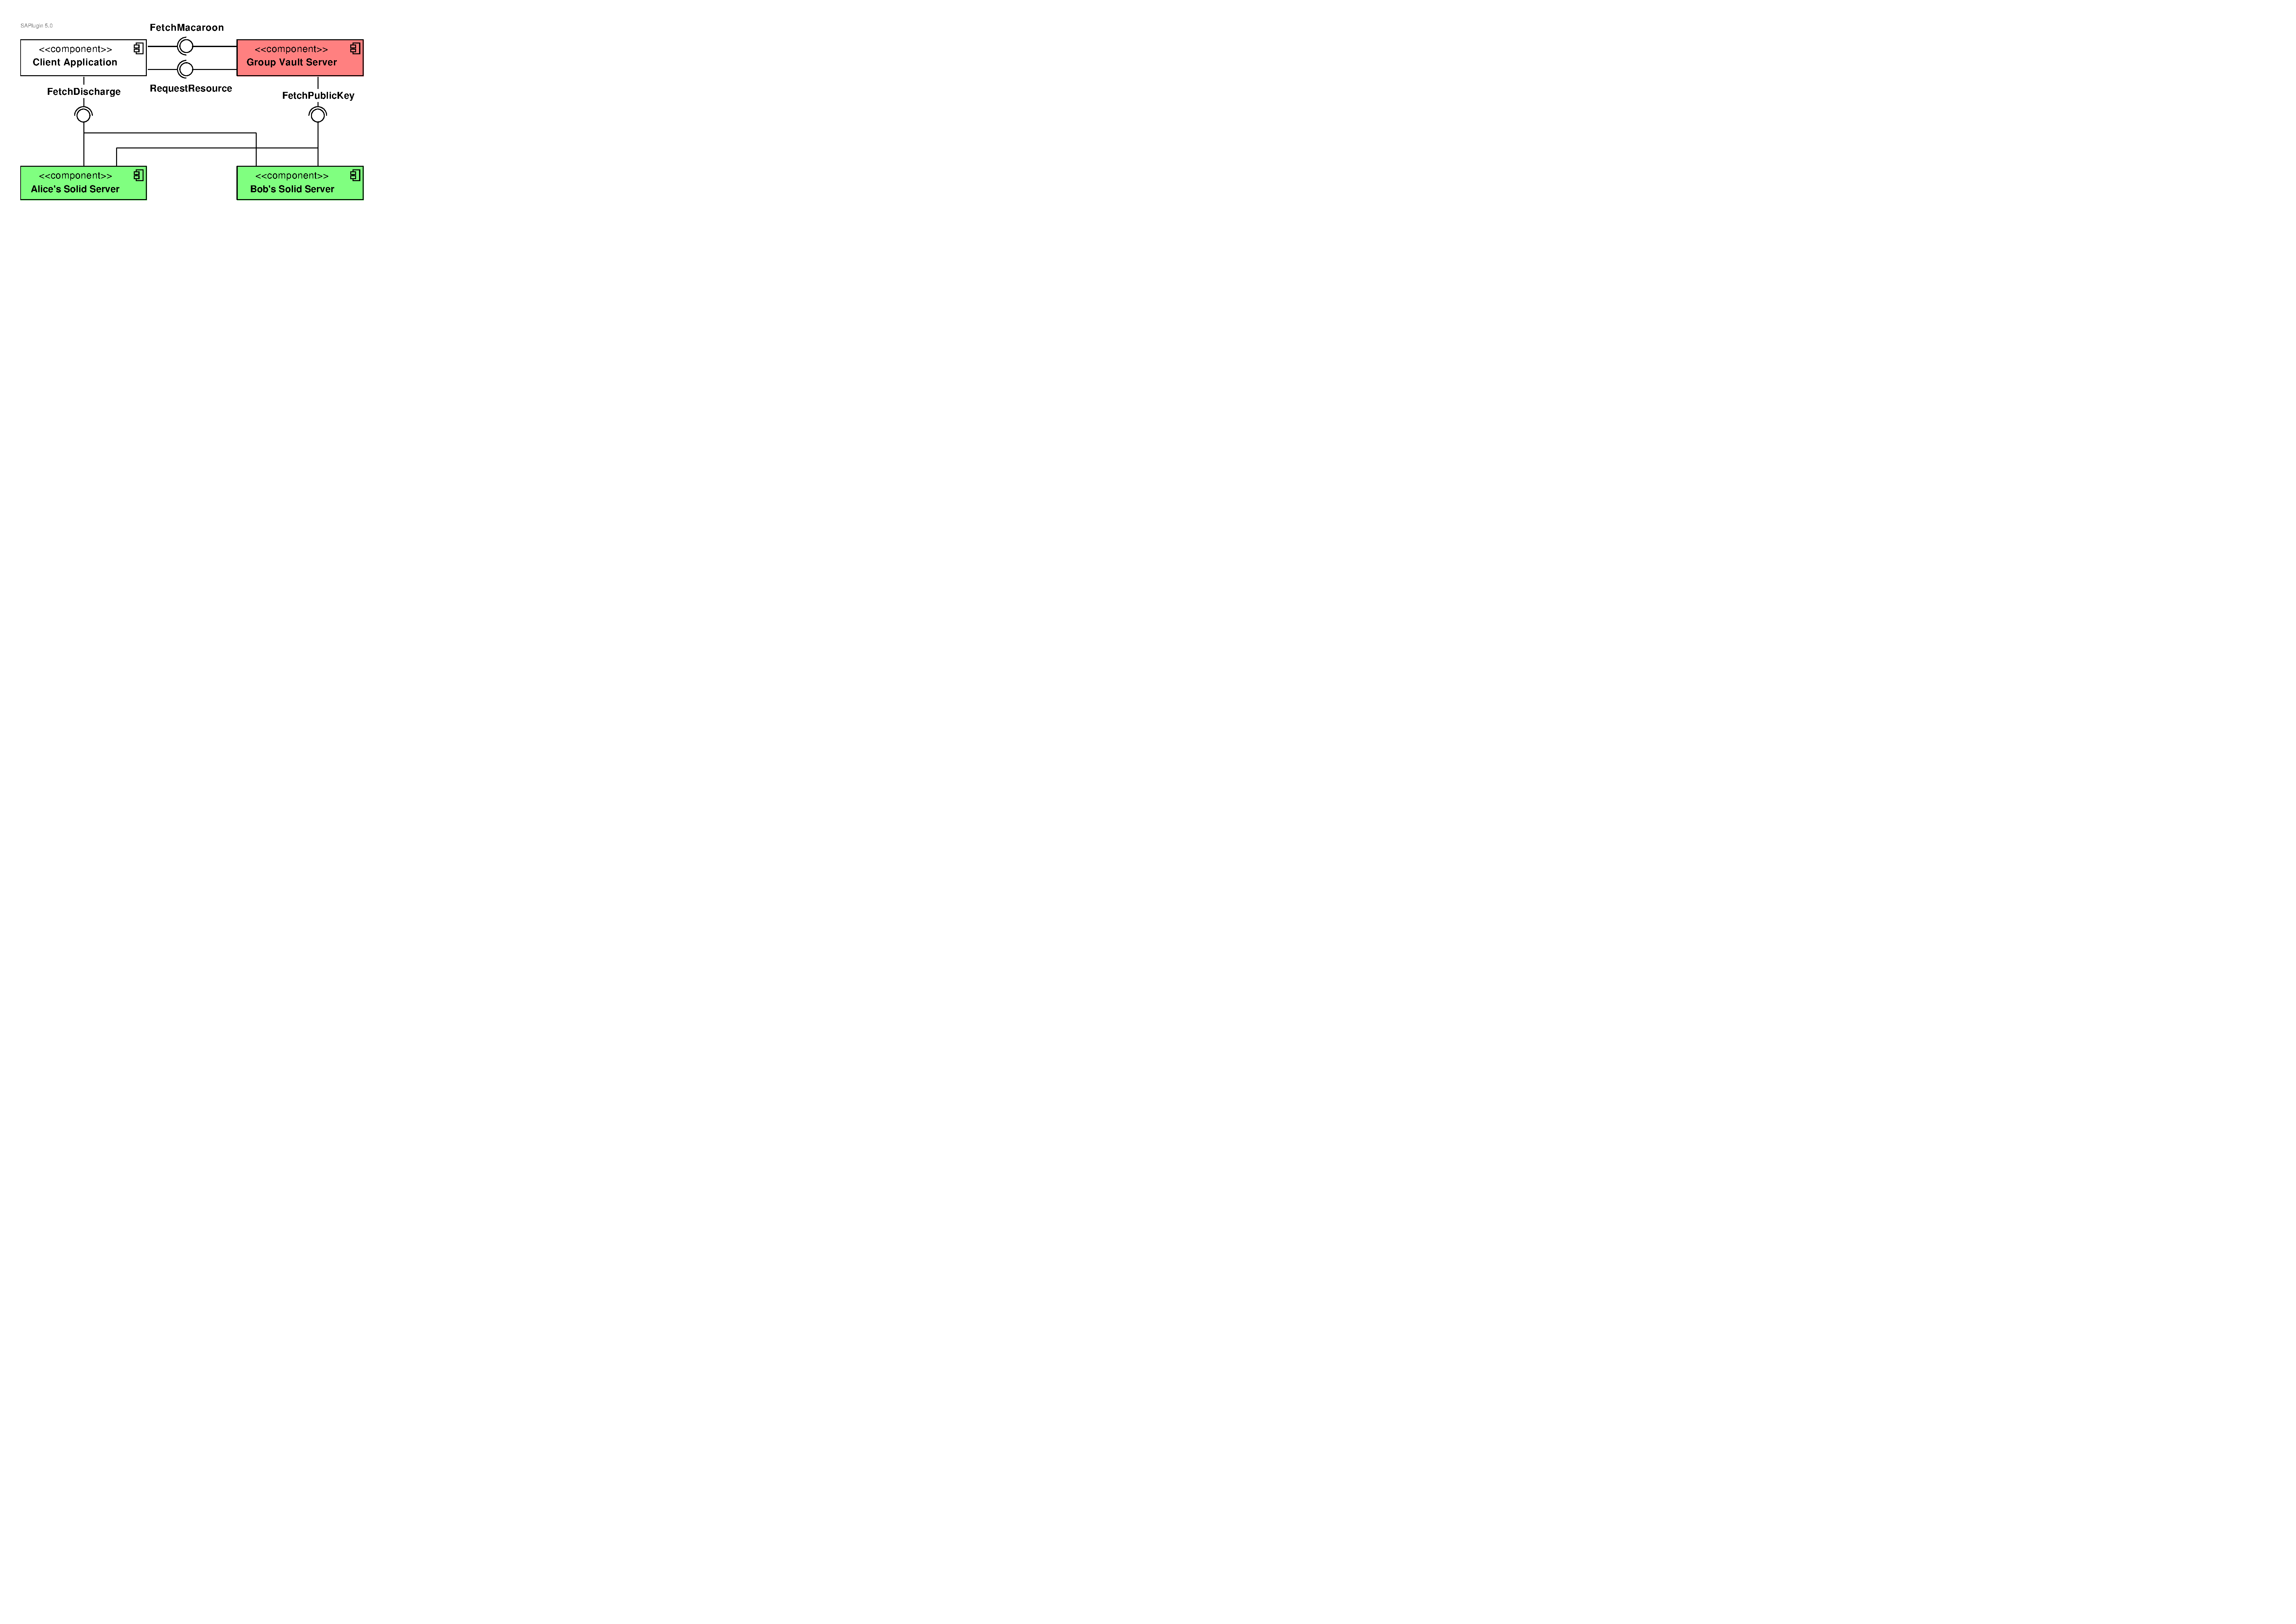
\includegraphics[width=0.50\textwidth]{images/macaroons-solid/ComponentDiagram-Group-Vault-System-Overview.pdf}
    \caption{System Overview of a Group Vault architecture.}
    \label{fig:gv-sys-overview}
\end{figure}

\begin{figure}[h]
    \centering
    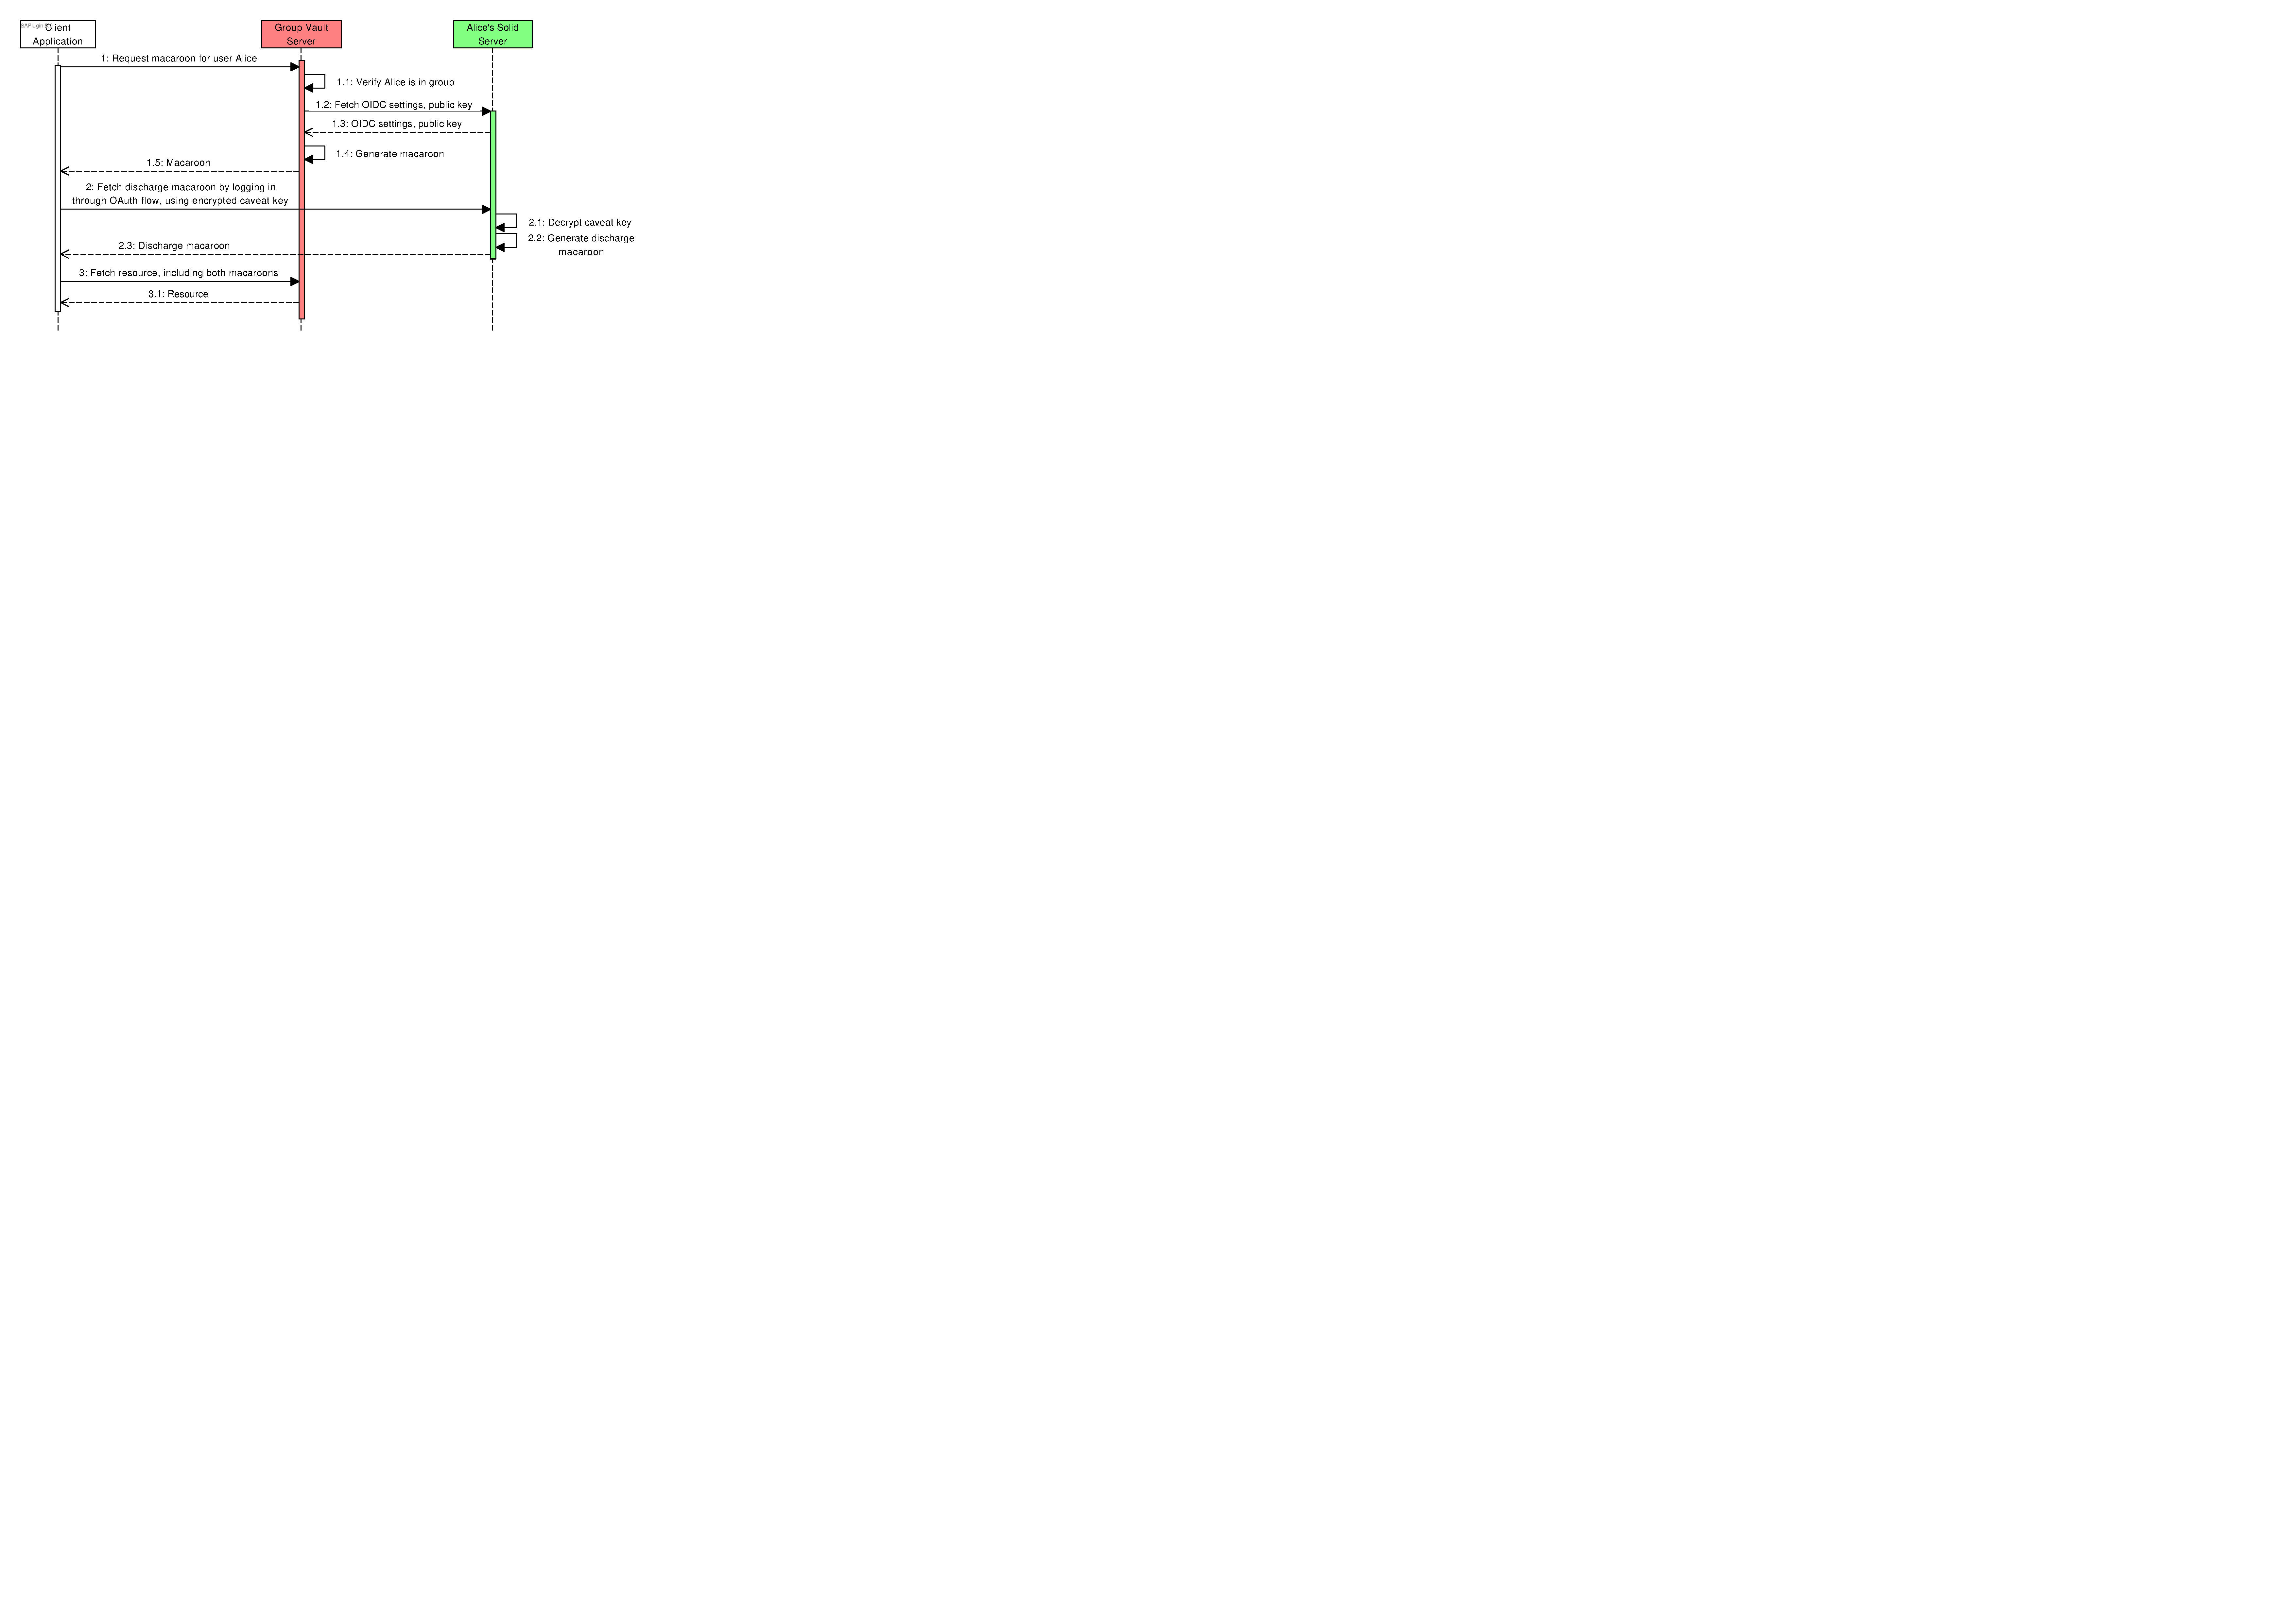
\includegraphics[width=1.0\textwidth]{images/macaroons-solid/InteractionDiagram-Group-Vault-Authentication-Flow.pdf}
    \caption{Authentication flow for accessing a resource from a \acrlong{GVS}.}
    \label{fig:gv-macaroon-flow}
\end{figure}

\begin{figure}[H]
    \centering
    {\fontfamily{qag}\selectfont }

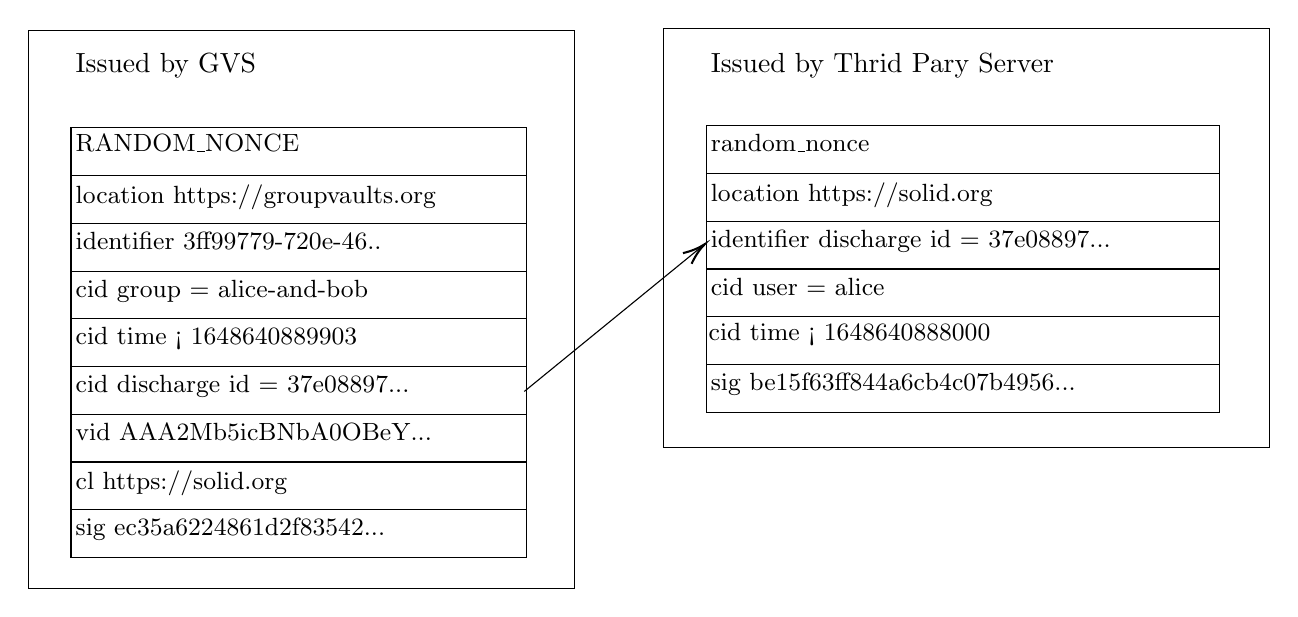
\begin{tikzpicture}[x=0.75pt,y=0.75pt,yscale=-1,xscale=1]
%uncomment if require: \path (0,331); %set diagram left start at 0, and has height of 331

%Shape: Rectangle [id:dp36106898781320174] 
\draw   (25,35) -- (288,35) -- (288,304) -- (25,304) -- cycle ;
%Shape: Rectangle [id:dp014069378908031283] 
\draw   (45.6,82) -- (265,82) -- (265,105) -- (45.6,105) -- cycle ;
%Shape: Rectangle [id:dp20345726322429547] 
\draw   (45.6,151) -- (265,151) -- (265,174) -- (45.6,174) -- cycle ;
%Shape: Rectangle [id:dp7088154428740524] 
\draw   (45.6,105) -- (265,105) -- (265,128) -- (45.6,128) -- cycle ;
%Shape: Rectangle [id:dp7951647364061636] 
\draw   (45.6,243) -- (265,243) -- (265,266) -- (45.6,266) -- cycle ;
%Shape: Rectangle [id:dp2294119235309251] 
\draw   (45.6,128) -- (265,128) -- (265,151) -- (45.6,151) -- cycle ;
%Shape: Rectangle [id:dp20892929793325288] 
\draw   (45.6,174) -- (265,174) -- (265,197) -- (45.6,197) -- cycle ;
%Shape: Rectangle [id:dp675591301361505] 
\draw   (45.6,266) -- (265,266) -- (265,289) -- (45.6,289) -- cycle ;
%Shape: Rectangle [id:dp946669631946771] 
\draw   (45.6,220) -- (265,220) -- (265,243) -- (45.6,243) -- cycle ;
%Shape: Rectangle [id:dp8118838011942326] 
\draw   (45.6,197) -- (265,197) -- (265,220) -- (45.6,220) -- cycle ;
%Shape: Rectangle [id:dp1748336079202455] 
\draw   (331,34) -- (623,34) -- (623,236) -- (331,236) -- cycle ;
%Shape: Rectangle [id:dp6959528817165129] 
\draw   (351.6,81) -- (599.08,81) -- (599.08,104) -- (351.6,104) -- cycle ;
%Shape: Rectangle [id:dp9148042784412247] 
\draw   (351.6,150) -- (599.08,150) -- (599.08,173) -- (351.6,173) -- cycle ;
%Shape: Rectangle [id:dp2637371441526388] 
\draw   (351.6,104) -- (599.08,104) -- (599.08,127) -- (351.6,127) -- cycle ;
%Shape: Rectangle [id:dp8589922967246587] 
\draw   (351.6,127) -- (599.08,127) -- (599.08,150) -- (351.6,150) -- cycle ;
%Shape: Rectangle [id:dp12106124639103755] 
\draw   (351.6,173) -- (599.08,173) -- (599.08,196) -- (351.6,196) -- cycle ;
%Shape: Rectangle [id:dp8847449056516175] 
\draw   (351.6,196) -- (599.08,196) -- (599.08,219) -- (351.6,219) -- cycle ;
%Straight Lines [id:da2707605121887615] 
\draw    (264,209) -- (349.45,139.26) ;
\draw [shift={(351,138)}, rotate = 140.78] [color={rgb, 255:red, 0; green, 0; blue, 0 }  ][line width=0.75]    (10.93,-3.29) .. controls (6.95,-1.4) and (3.31,-0.3) .. (0,0) .. controls (3.31,0.3) and (6.95,1.4) .. (10.93,3.29)   ;

% Text Node
\draw (46.6,45) node [anchor=north west][inner sep=0.75pt]   [align=left] {Issued by \acrlong{GVS}};
% Text Node
\draw (46.6,84) node [anchor=north west][inner sep=0.75pt]   [align=left] {{\small RANDOM\_NONCE}};
% Text Node
\draw (46.6,108) node [anchor=north west][inner sep=0.75pt]   [align=left] {{\small location https://groupvaults.org}};
% Text Node
\draw (46.6,131) node [anchor=north west][inner sep=0.75pt]  [font=\small] [align=left] {identifier 3ff99779-720e-46..};
% Text Node
\draw (46.6,154) node [anchor=north west][inner sep=0.75pt]  [font=\small] [align=left] {cid group = alice-and-bob};
% Text Node
\draw (46.6,177) node [anchor=north west][inner sep=0.75pt]  [font=\small] [align=left] {cid time < 1648640889903};
% Text Node
\draw (46.6,200) node [anchor=north west][inner sep=0.75pt]  [font=\small] [align=left] {cid discharge id = 37e08897...};
% Text Node
\draw (46.6,223) node [anchor=north west][inner sep=0.75pt]  [font=\small] [align=left] {vid AAA2Mb5icBNbA0OBeY...};
% Text Node
\draw (46.6,246) node [anchor=north west][inner sep=0.75pt]  [font=\small] [align=left] {cl https://solid.org};
% Text Node
\draw (46.6,269) node [anchor=north west][inner sep=0.75pt]  [font=\small] [align=left] {sig ec35a6224861d2f83542...};
% Text Node
\draw (352.6,45) node [anchor=north west][inner sep=0.75pt]   [align=left] {Issued by Thrid Pary Server};
% Text Node
\draw (352.6,84) node [anchor=north west][inner sep=0.75pt]  [font=\small] [align=left] {random\_nonce};
% Text Node
\draw (352.6,107) node [anchor=north west][inner sep=0.75pt]  [font=\small] [align=left] {location https://solid.org};
% Text Node
\draw (352.6,130) node [anchor=north west][inner sep=0.75pt]  [font=\small] [align=left] {identifier discharge id = 37e08897...};
% Text Node
\draw (352.6,153) node [anchor=north west][inner sep=0.75pt]  [font=\small] [align=left] {cid user = alice};
% Text Node
\draw (351.6,175) node [anchor=north west][inner sep=0.75pt]  [font=\small] [align=left] {cid time < 1648640888000};
% Text Node
\draw (352.6,199) node [anchor=north west][inner sep=0.75pt]  [font=\small] [align=left] {sig be15f63ff844a6cb4c07b4956...};
\end{tikzpicture}
    \caption{Example group vault macaroon and related discharge macaroon.}
    \label{fig:gv-macaroon-example}
\end{figure}

\section{Decentralized delegation of access tokens}
\label{sec:decentralized-delegation}
A second problem in the context of secure data aggregation is delegation of access tokens. In the case of more complex aggregations, there is often more than one node performing the aggregation. Another possibility is that a component performing data aggregations also needs data from another component or service, which also needs access to the user's pod. 

\subsection{Existing access token delegation mechanisms}
Methods for delegating access tokens already exist, even within the OAuth standard. An example is the OAuth On-Behalf-Of flow\footnote{\label{fn:obo}See \url{https://docs.microsoft.com/en-us/azure/active-directory/develop/v2-oauth2-on-behalf-of-flow}}. This flow supports the delegation of an access token of \textit{Service A} to \textit{Service B}, propagating the access token's bound identity and permissions. This concept is called \textit{access token delegation} because Service B acts on Service A's behalf and in its name. 

The On-Behalf-Of flow works as illustrated in figure \ref{fig:obo-flow} (protocol description based on (\ref{fn:obo})). 

\begin{figure}[H]
    \centering
   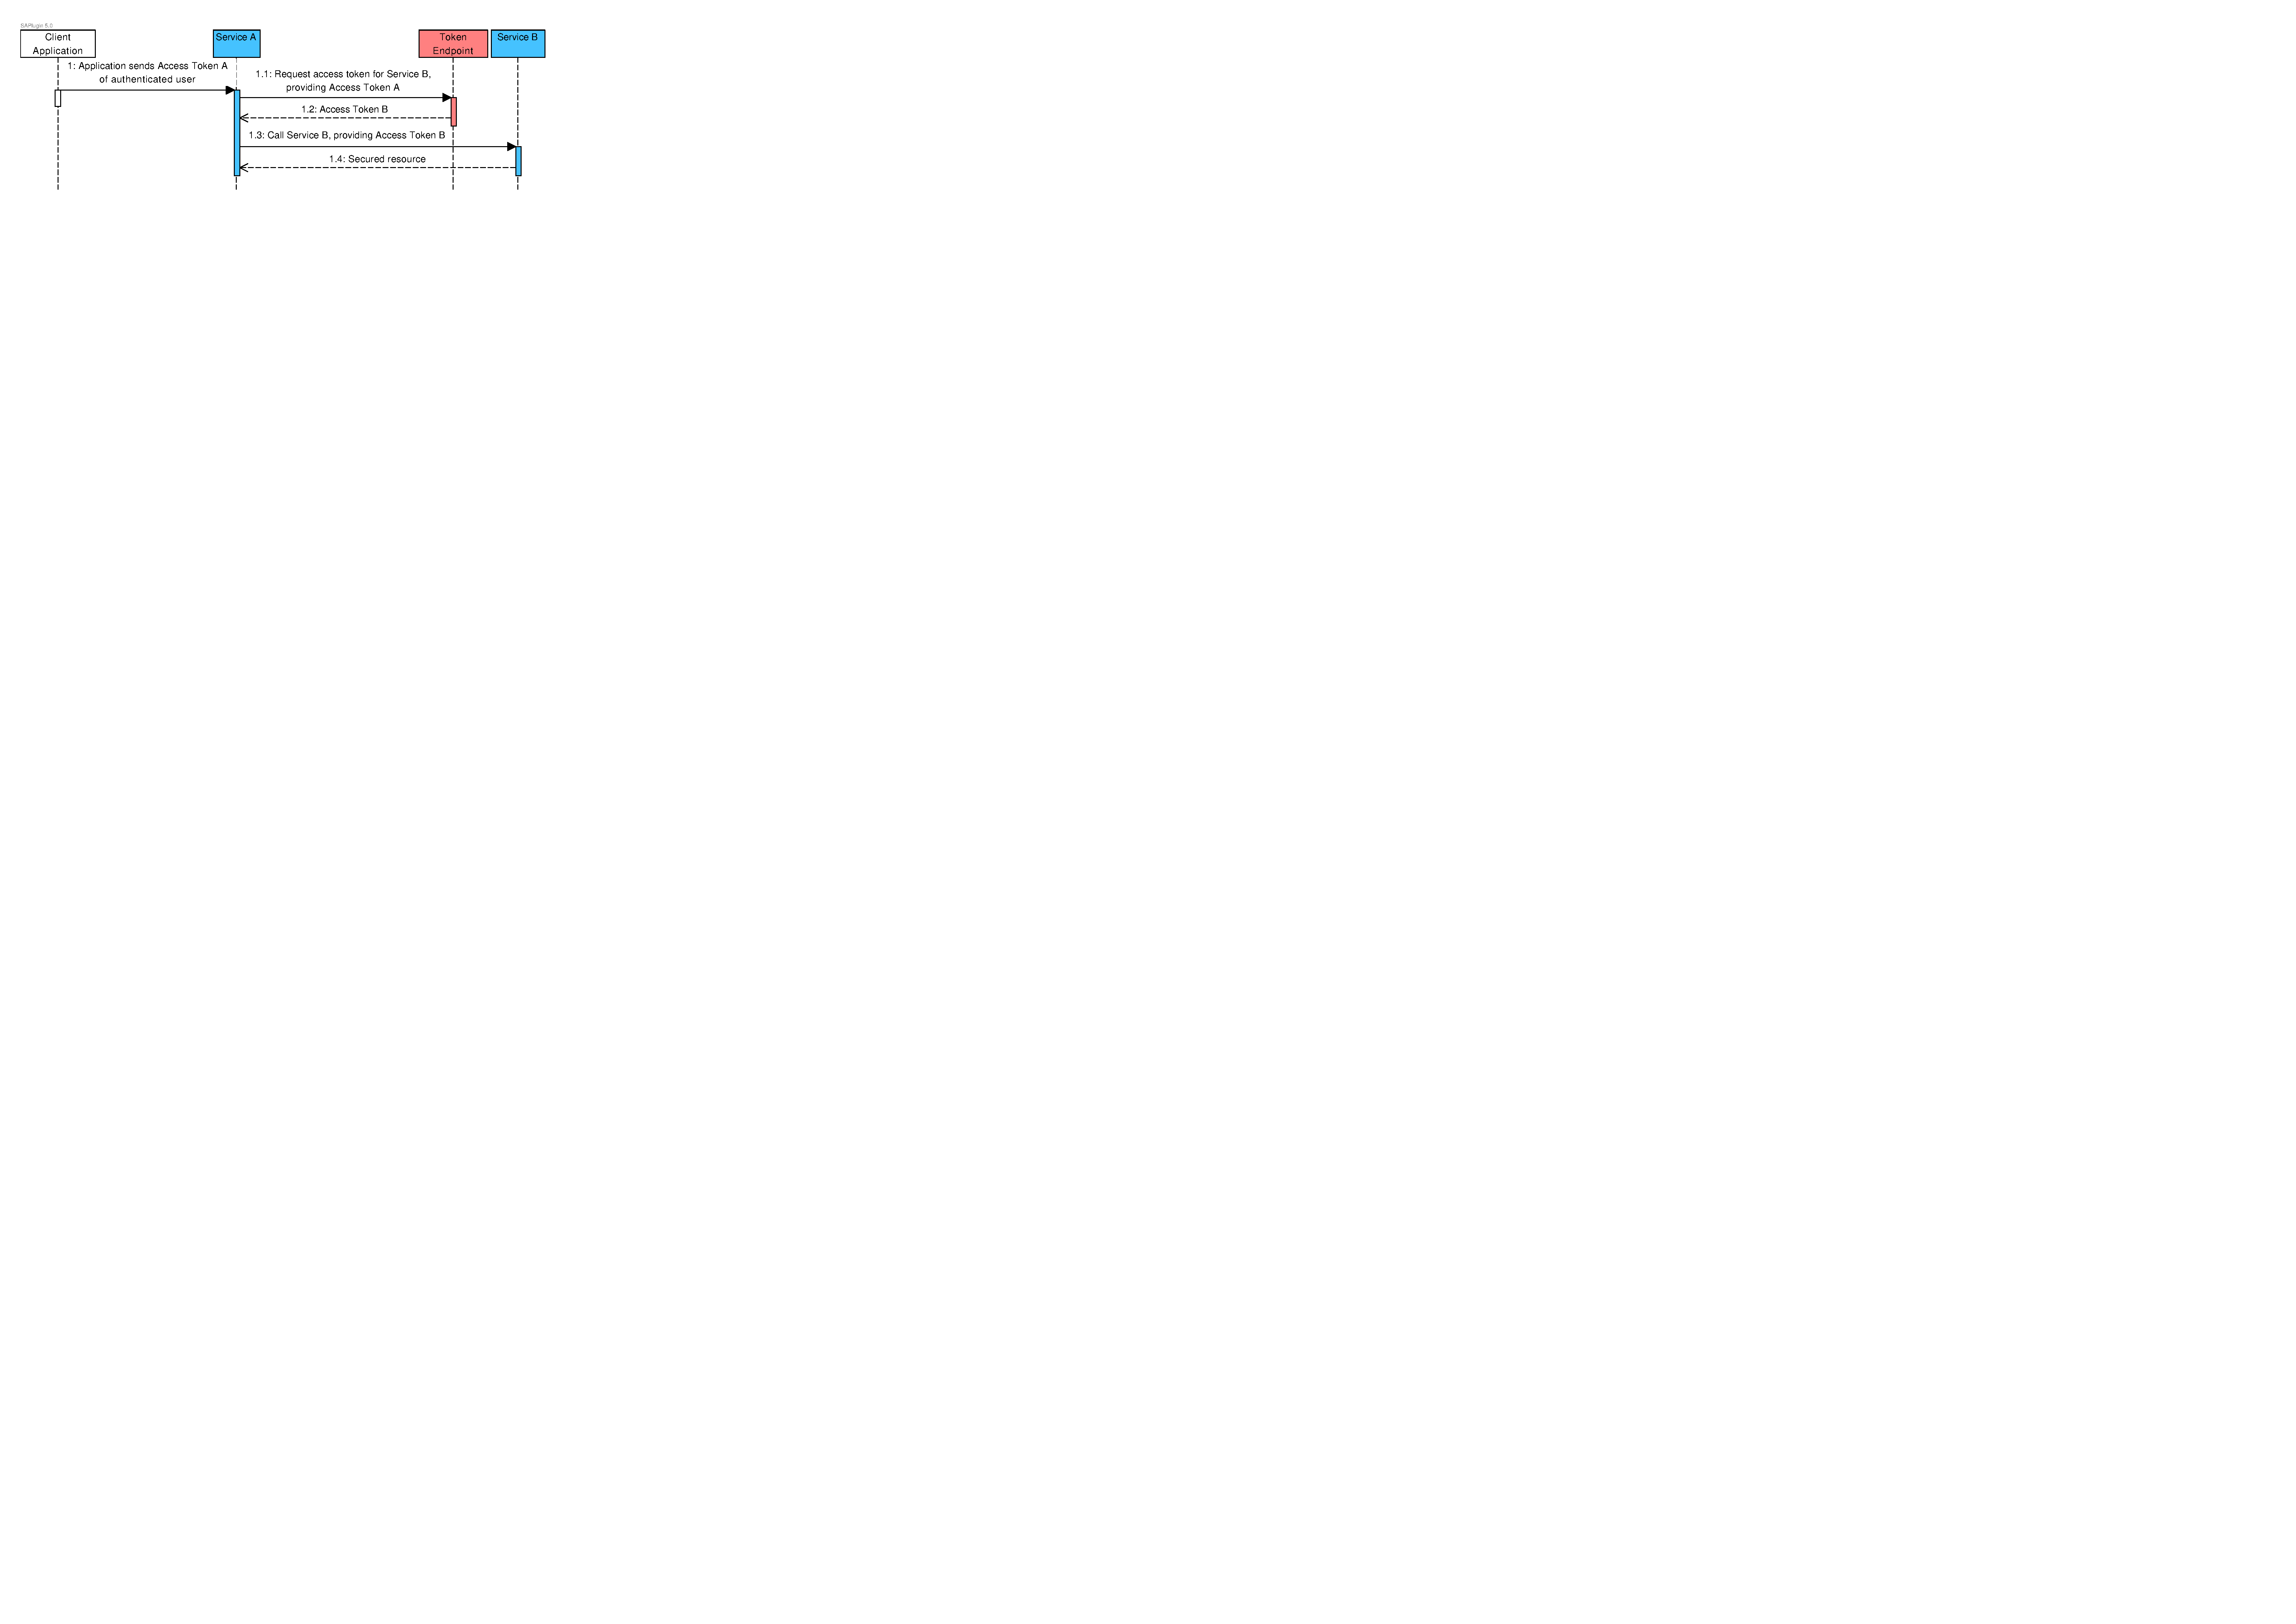
\includegraphics[width=1.0\textwidth]{images/macaroons-solid/InteractionDiagram-OBO-Flow.pdf}
    \caption{OAuth On-Behalf-Of flow}
    \label{fig:obo-flow}
\end{figure}

\noindent Concretely, the following steps are executed:
\begin{enumerate}
    \item The client has authenticated the user and has an access token bound to this user's identity (Access Token A)
    \item The client sends a request to Service A, providing Access Token A
    \item Service A requests an access token for Service B on behalf of itself, providing Access Token A as part of the request
    \item The Token Endpoint generates an access token, B, and returns it
    \item Service A calls Service B, including Access Token B in the request
    \item Service B returns the secured resource
\end{enumerate}
\noindent Although this method functionally works, it has a number of important limitations in a decentralized environment. The main limitation is that this flow relies heavily on the Token Endpoint to generate new tokens every time an access token needs to be delegated. This creates a bottleneck when such tokens must often be generated, and makes the system more centralized. 

\newpage
\subsection{Decentralized delegation of access tokens using macaroons}
Macaroons have a number of interesting properties that make them suitable as an access token for realizing decentralized delegation of access token. Concretely, this decentralized delegation means that a Service A can delegate its access token to Service B, without having to contact the Token Endpoint for obtaining a new token.

Delegation of macaroons works out-of-the-box, because by default macaroons are not bound to a specific client (nor is a proof-of-possession mechanism employed). Such restrictions must be added by adding caveats that restrict the macaroon's usage to a specific application (and a specific user, target resource, etc.). By default, macaroons can also be extended with additional caveats. This enables a service that wishes to delegate its access token to add additional constraints on the token usage (such as making it usable only once, adding a more strict time restriction, etc.).

Since Solid uses OAuth as its authentication mechanism, a new access token mechanism should be compatible with OAuth. Fortunately, macaroons have already been used in production systems as access and refresh tokens. The original macaroons paper discusses macaroons in the context of OAuth \citep[p.12]{macaroons}, and the ForgeRock AM 7 Access Management system supports the use of macaroons as access tokens in OAuth\footnote{See \url{https://backstage.forgerock.com/docs/am/7/oauth2-guide/oauth2-macaroons.html}}.

Realizing access delegation naively may lead to severe vulnerabilities, where tokens can be stolen. Therefore, delegation should be disabled by default by limiting a macaroon to a certain WebID (the application's WebID). An application that requests access delegation should include this information when requesting an access token, specifying the WebIDs of the third-party services. 

Figure \ref{fig:decentralized-delegation-macaroon} illustrates the flow of delegating an access token in Solid, in the context of an aggregator.

\begin{figure}[H]
    \centering
   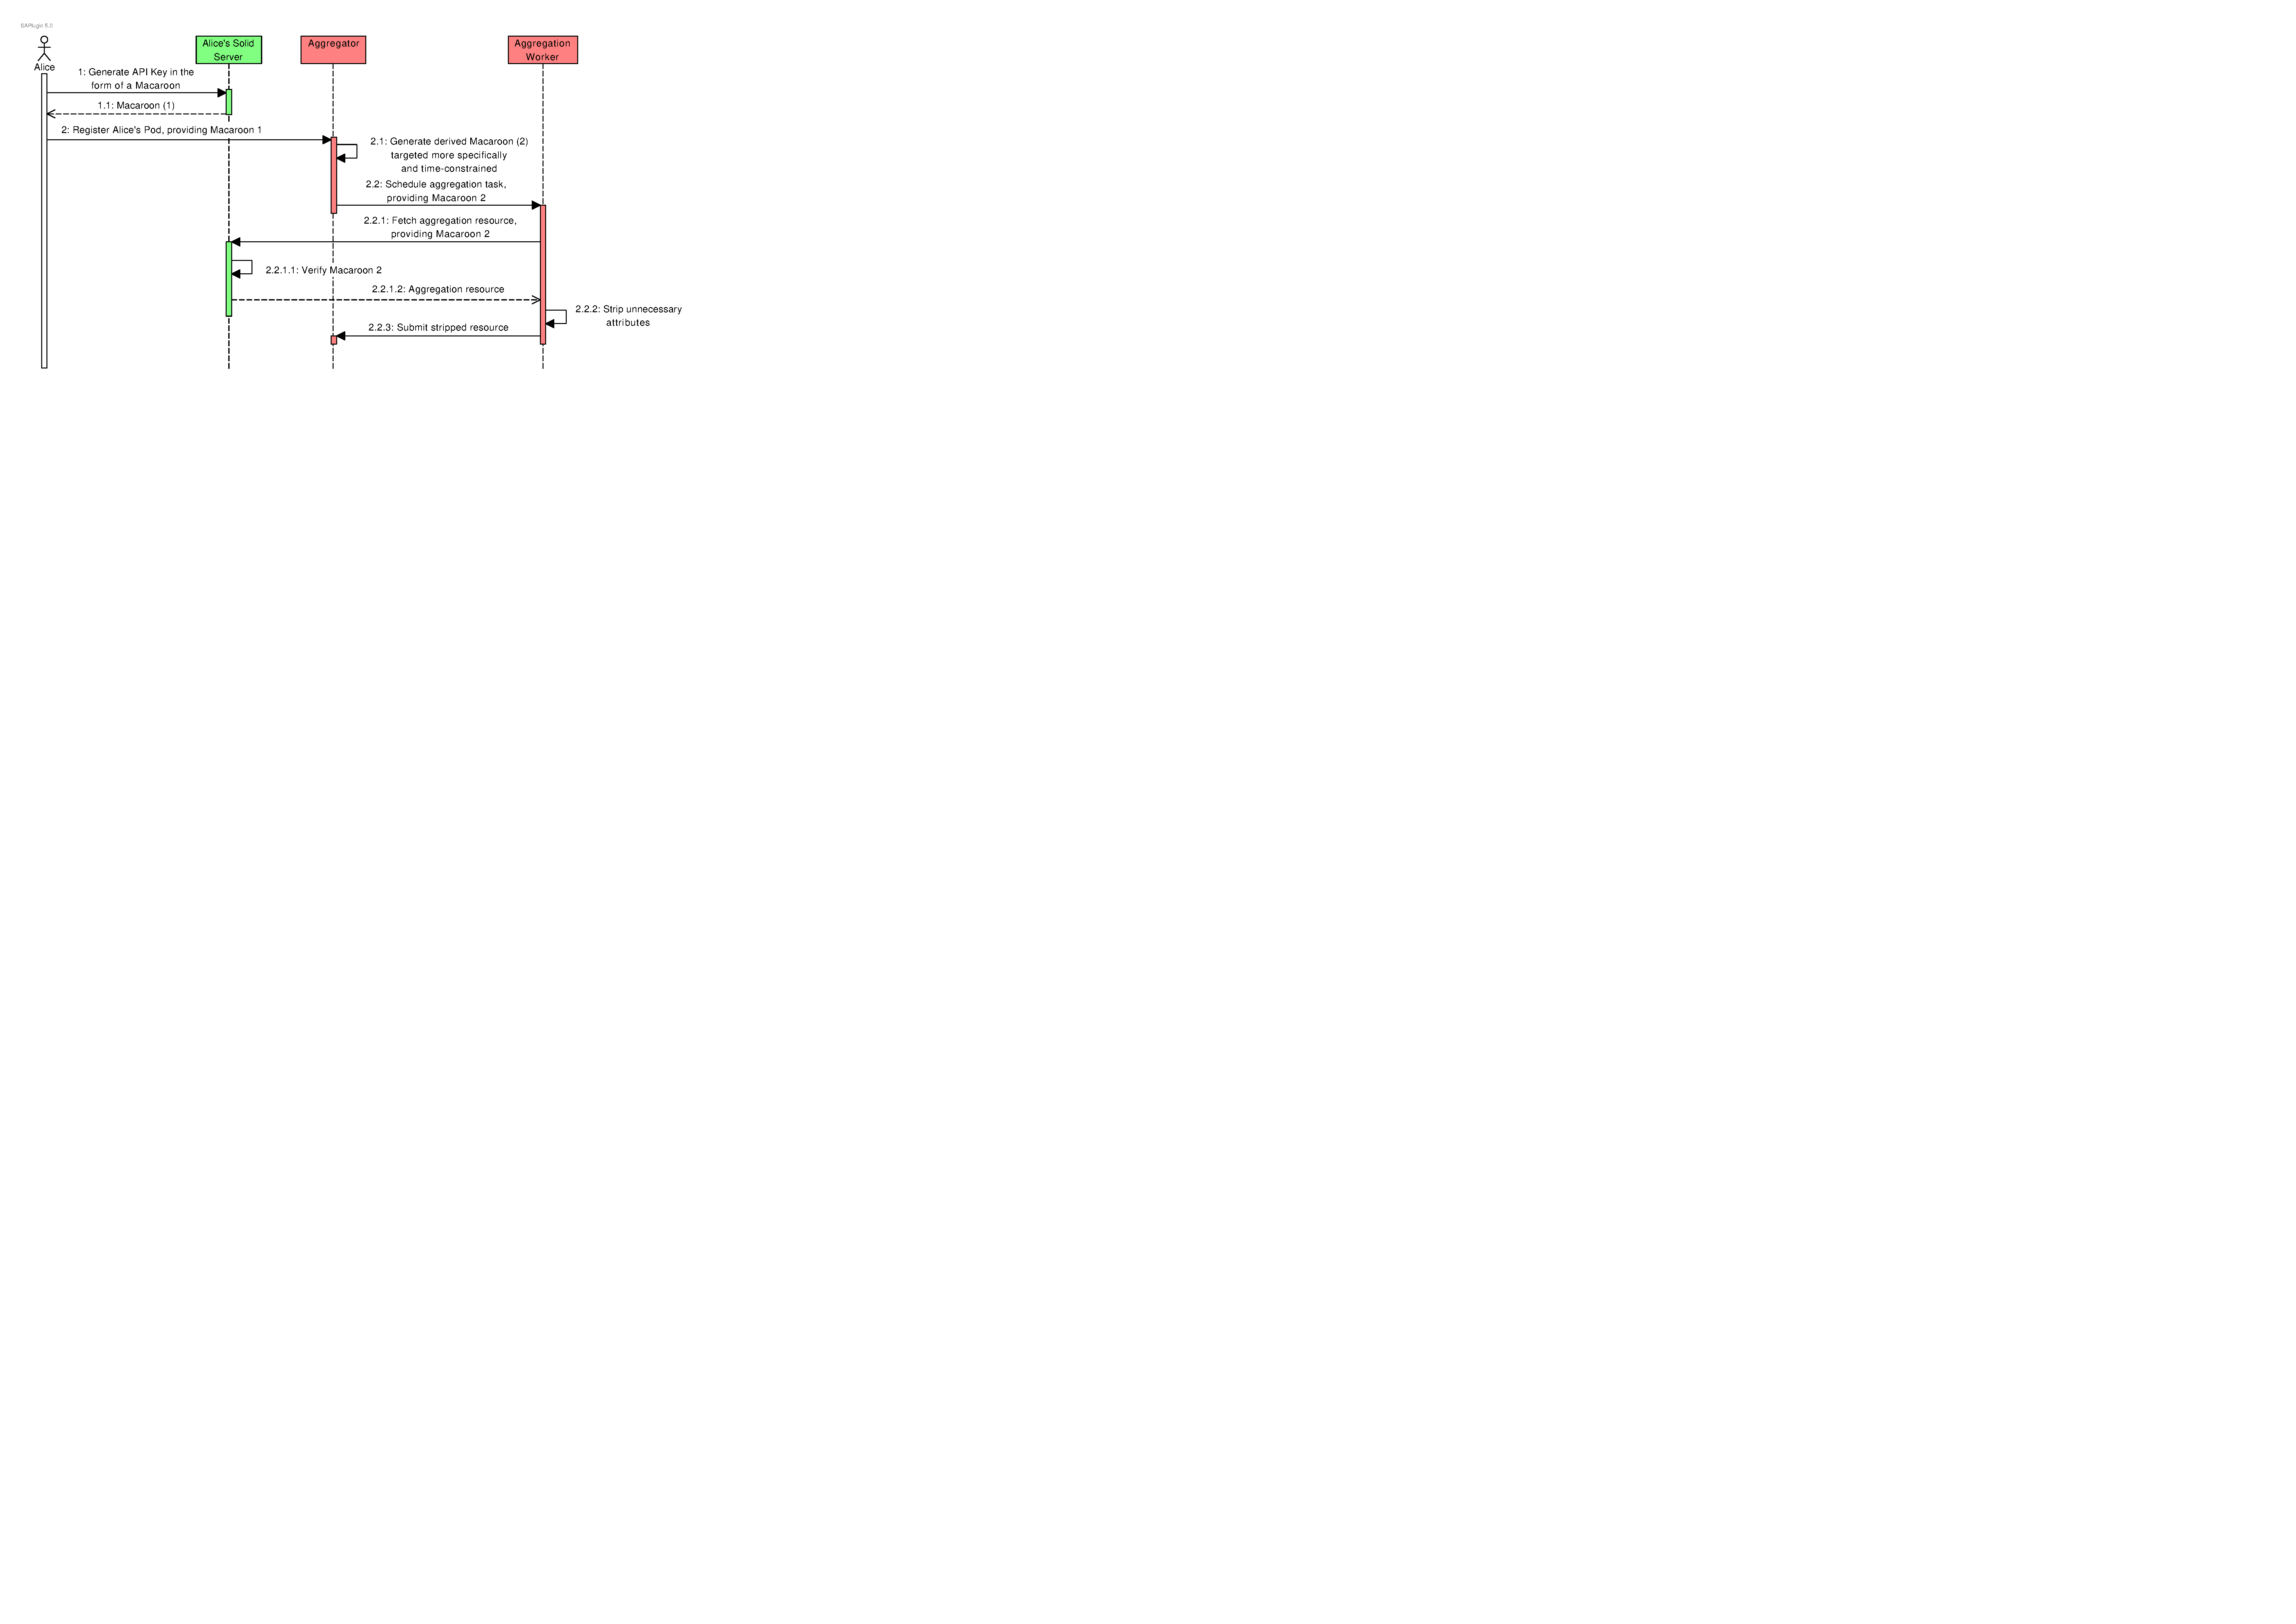
\includegraphics[width=1.0\textwidth]{images/macaroons-solid/InteractionDiagram-Decentralized-Delegation-of-Macaroon.pdf}
    \caption{Decentralized Delegation of Macaroon in Solid Data Aggregator}
    \label{fig:decentralized-delegation-macaroon}
\end{figure}

\noindent As can be seen in figure \ref{fig:decentralized-delegation-macaroon}, the \texttt{Aggregator} component does not need to contact \texttt{Alice's Solid Server} (the token endpoint) to generate a new macaroon to pass to the \texttt{AggregationWorker}. 

Apart from not having to contact the token endpoint, the usage of macaroons in this context provides additional benefits as well. 
Firstly, when the \texttt{Aggregator} derives a new macaroon to delegate, this can be confined to the concrete request very precisely. For instance, the derived macaroon can be limited to a specific resource (such as \texttt{health-data/01042022.json}), to a specific method (such as \texttt{GET}), and within a very specific time frame (such as in the next sixty seconds). 

Additionally, combining macaroons with the privacy filters proposed in chapter \ref{cha:privacy-filters} also allows confining the tokens to a specific privacy level. In this way, a Solid server can rewrite the data to strip sensitive personal information even before passing it to the aggregator. This decreases the reliance on the aggregator to correctly perform such operations, increasing the trust level of aggregators. Furthermore, by already stripping a number of attributes in the Solid server, the system load of the aggregator is decreased since it must receive less data.

Finally, macaroons also prove to be a very safe and secure method of handing out API keys. Traditionally, API keys (whether they are in the form of bearer tokens, \gls{JWT}s or other token types) require either extensive bookkeeping (in the case of bearer tokens) or verifying signatures (in the case of \gls{JWT}s) to verify whether they are valid. However, none of them offer good anti-theft mechanisms apart from token revocation. Unfortunately, such token thefts can often go unnoticed. However, since macaroons can be easily confined to an identifier (such as an IP address), they offer more extensive protection mechanisms. They also don't come with the downside of extensive bookkeeping for bearer tokens (since authorization limitations are embedded in the macaroon), and can be revoked easily by adding a caveat to check the token identifier in a revocation list.

Concretely, the content of Macaroon 1 and Macaroon 2 would look like the macaroons presented in table \ref{table:delegated-macaroon}.

\begin{table}[!htb]
   \centering
    \begin{subtable}{.4\linewidth}
      \centering
        \begin{tabular}{|l|}
        \hline
        RANDOM\_NONCE                                       \\ \hline
        location https://pods.org                           \\ \hline
        identifier 3ff99779-720e...                         \\ \hline
        cid user = alice                                    \\ \hline
        cid operation = read                                \\ \hline
        cid target = /health                                \\ \hline
        cid expiry = 01-01-2024                             \\ \hline
        cid webid = https://agg.com/...                     \\ \hline
        cid privacy\_level = 3                              \\ \hline
        sig ec35a6224861d2f83542c7f2...                     \\ \hline
        \end{tabular}
        \caption{Aggregator macaroon}
    \end{subtable}%
    \begin{subtable}{.6\linewidth}
      \centering
        \begin{tabular}{|l|}
        \hline
        RANDOM\_NONCE                                       \\ \hline
        location https://pods.org                           \\ \hline
        identifier 3ff99779-720e...                         \\ \hline
        cid user = alice                                    \\ \hline
        cid operation = read                                \\ \hline
        cid target = /health/010422.json                    \\ \hline
        cid expiry = 01-06-2022 17:04:02                    \\ \hline
        cid webid = https://agg.com/...                     \\ \hline
        cid privacy\_level = 3                              \\ \hline
        cid ip = 193.190.253.145                            \\ \hline
        sig b7da027f072ce6f5a64c35ab...                     \\ \hline
        \end{tabular}
        \caption{Derived macaroon}
    \end{subtable} 
    \caption{Illustration of macaroon delegation}
    \label{table:delegated-macaroon}
\end{table}
